%
%
\documentclass[twoside,11pt]{../sty/report_petsc}

\usepackage{makeidx,xspace}
\usepackage[bookmarksopen,colorlinks]{hyperref}
\usepackage[all]{hypcap}
\usepackage{color}
\input pdfcolor.tex

\usepackage[pdftex]{graphicx}


\usepackage{times}
\usepackage{listings}
\usepackage{tikz}
%\usepackage{psfig}
\usepackage{../sty/verbatim}
\usepackage{../sty/tpage}
\usepackage{../sty/here}
\usepackage{../sty/anlhelper}
\usepackage[hyphens,spaces,obeyspaces]{../sty/trl}

\setlength{\textwidth}{6.5in}
\setlength{\oddsidemargin}{0.0in}
\setlength{\evensidemargin}{0.0in}
\setlength{\textheight}{9.2in}
\setlength{\topmargin}{-.8in}

\newcommand{\findex}[1]{\index{#1}}
\newcommand{\sindex}[1]{\index{#1}}
\newcommand{\A}{\mbox{\boldmath \(A\)}}
\newcommand{\F}{\mbox{\boldmath \(F\)}}
\newcommand{\J}{\mbox{\boldmath \(J\)}}
\newcommand{\x}{\mbox{\boldmath \(x\)}}
\newcommand{\bb}{\mbox{\boldmath \(b\)}}
\newcommand{\rr}{\mbox{\boldmath \(r\)}}
hyperbaseurl

\makeindex

% Defines the environment where design issues are discussed. In the manual
% version of this report, these regions are ignored.
\def\design{\medskip \noindent Design Issue:\begin{em}}
\def\enddesign{\end{em} \medskip}
% Manual version:
% \def\design{\comment}
% \def\enddesign{\endcomment}

% Print DRAFT in large letters across every page
%\special{!userdict begin /bop-hook{gsave 200 70 translate
%65 rotate /Times-Roman findfont 216 scalefont setfont
%0 0 moveto 0.95 setgray (DRAFT) show grestore}def end}

% Defines that we're doing the whole manual, not the short intro part,
% used in part1.tex.
\def\shortintro{false}

\usepackage{fancyhdr,lastpage}
\pagestyle{fancy}
\rhead{PETSc 3.5 \today}

\begin{document}


%%%%%%%%%%%%%%%%%%%%%%%%%%%%%%%%%%%%%%%%%%%%%%%%%%%%%%%%%%%%%%%%%%%%%%%%%%%%%%%%%%%%

\pagestyle{empty}
\hspace{-.65in}
\includegraphics{ArgonneLogo}
\hfill  {\large {\bf ANL-95/11 Rev 3.5}}

\vspace*{3in}
\noindent {\huge{\bf PETSc Users Manual}}
\vspace*{8pt}
\hrule
\vspace*{8pt}
\noindent {\Large{\it Revision 3.5}}

\vspace*{1in}
\noindent \\
{\Large {\bf Mathematics and Computer Science Division}}

\vspace*{10pt}


\vspace*{20pt}


%%%%%%%%%%%%%%%%%%%%%%%%%%%%%%%%%%%%%%%%%%%%%%%%%%%%%%%%%%%%%%%%%%%%%%%%%%%%%%%%%%%%

\newpage
\centerline{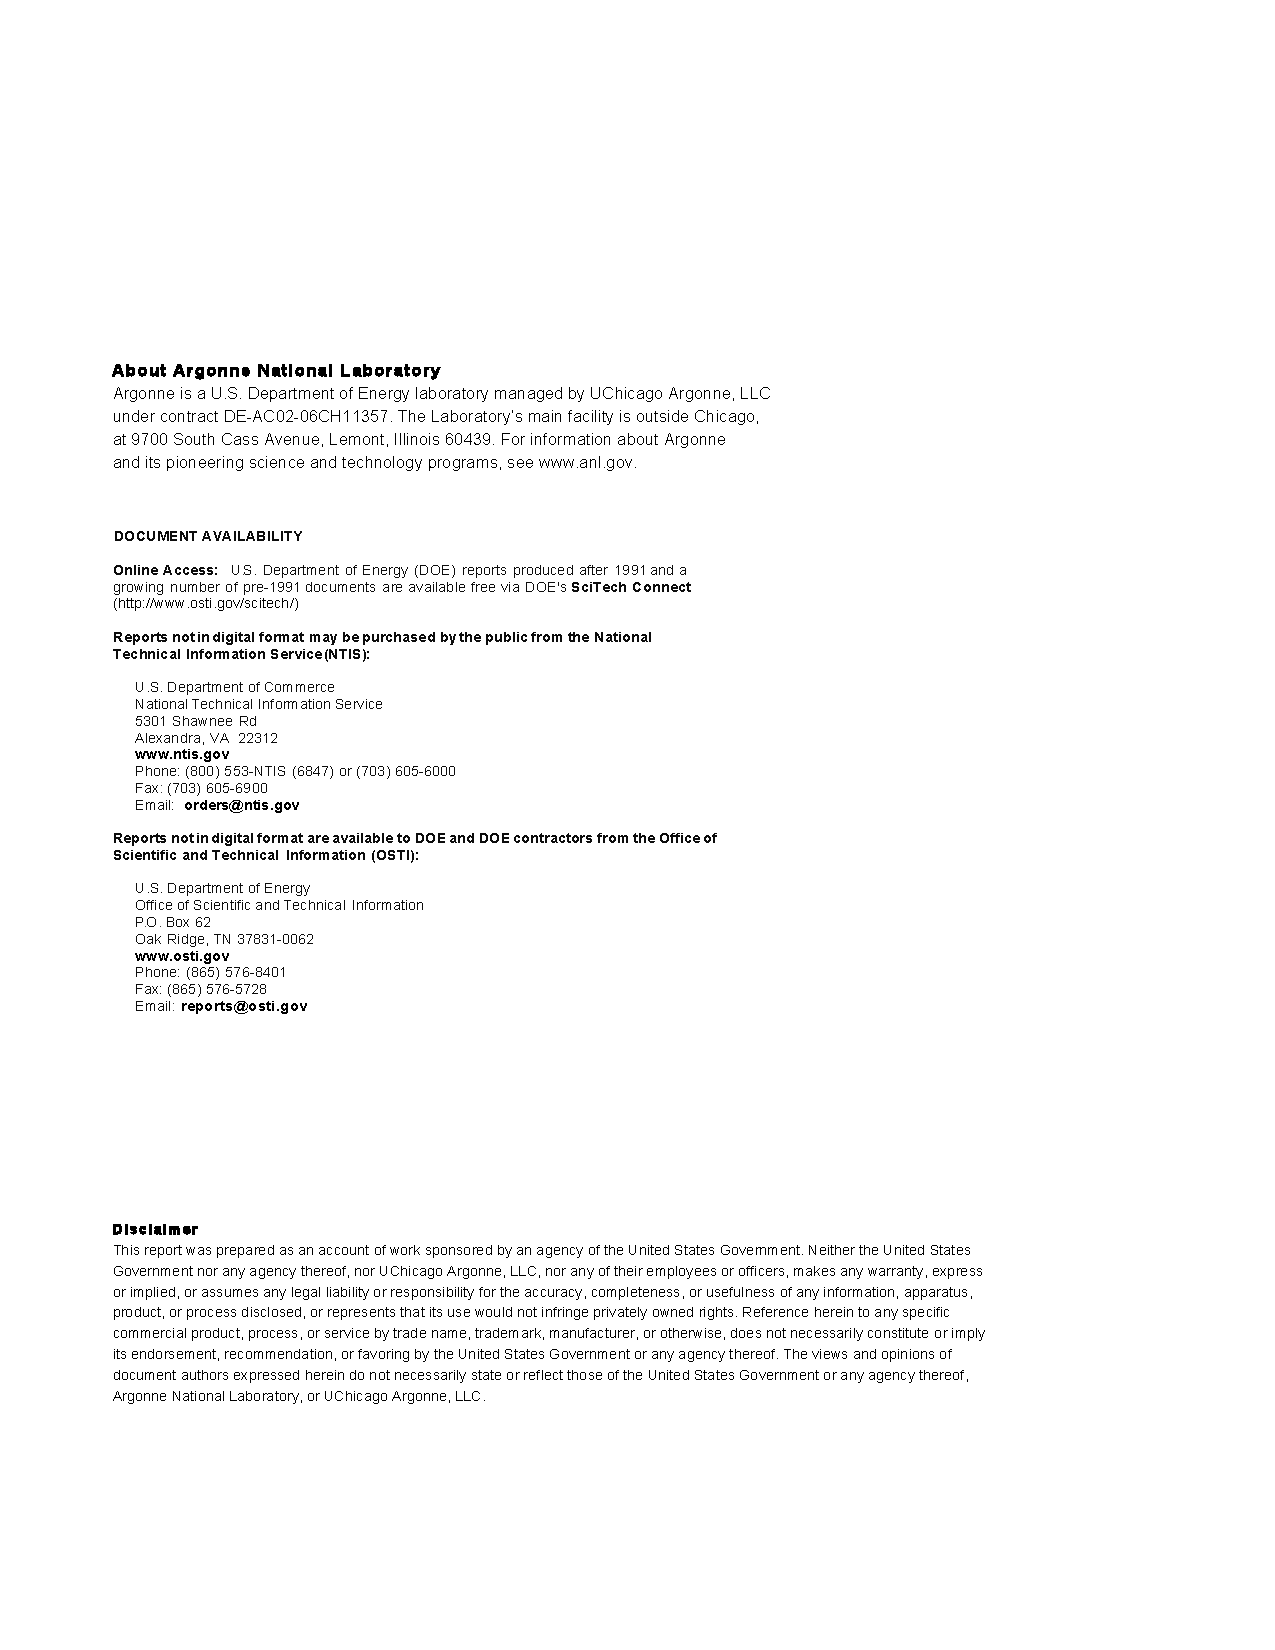
\includegraphics{ArgonneReportTemplatePage2}}
\newpage

\hfill {\large {\bf ANL-95/11 Rev 3.5}}

\vspace*{3in}
\noindent {\LARGE{\bf PETSc Users Manual}}
\vspace*{8pt}
\hrule
\vspace*{8pt}
\noindent {\Large{\it Revision 3.5}}

\vspace*{1in}
\noindent Prepared by \\
S. Balay, S. Abhyankar, M. Adams, J. Brown, P. Brune, K. Buschelman, V. Eijkhout, W. Gropp, D. Kaushik, \\
M. Knepley, L. Curfman McInnes, K. Rupp, B. Smith, and H. Zhang \\
Mathematics and Computer Science Division, Argonne National Laboratory

\vspace*{30pt}
\noindent June 2014

\vspace*{20pt}
\noindent This work was supported by the Office of Advanced Scientific Computing Research, \\
Office of Science, U.S. Department of Energy, under Contract DE-AC02-06CH11357.


\cleardoublepage
%\pagestyle{plain}
\pagestyle{fancy}
\vspace{1in}
\date{\today}

% Abstract for users manual
\addcontentsline{toc}{chapter}{Abstract}
% Abstract for TAO Users Manual

\addcontentsline{toc}{chapter}{Preface}
\section*{Preface}

The Toolkit for Advanced Optimization (TAO) focuses on the development
of algorithms and software for the solution of large-scale optimization 
problems on high-performance architectures.  Areas of interest include 
unconstrained and bound-constrained optimization, nonlinear least squares 
problems, optimization problems with partial differential equation 
constraints, and variational inequalities and complementarity 
constraints.

The development of TAO was motivated by the scattered support for
parallel computations and the lack of reuse of external toolkits in
current optimization software.  Our aim is to produce high-quality 
optimization software for computing environments ranging from 
workstations and laptops to massively parallel high-performance 
architectures.  Our design decisions are strongly motivated by 
the challenges inherent in the use of large-scale distributed 
memory architectures and the reality of working with large, 
often poorly structured legacy codes for specific 
applications.

This manual describes the use of TAO 2.2.0.  Since TAO is still under 
development, changes in usage and calling sequences may occur.  TAO 
is fully supported; see the the web site \url{http://www.mcs.anl.gov/tao} 
for information on contacting the developers.

%%% Local Variables: 
%%% mode: latex
%%% TeX-master: "manual_tex"
%%% End: 



\cleardoublepage


% ---------------------------------------------------------------------------
%

\medskip\medskip

\noindent {\bf Getting Information on PETSc:} 

\medskip


\noindent {\bf On-line:}
\begin{list}{$\bullet$}
{
\setlength{\itemsep}{-.020in} 
\setlength{\topsep}{0in} 
\setlength{\partopsep}{0in}
}
\item Manual pages for all routines, including example usage
\begin{list}{$\bullet$}
{
\setlength{\itemsep}{-.020in} 
\setlength{\topsep}{0in} 
\setlength{\partopsep}{0in}
}
   \item \trllink{index.html}{docs/index.html} in the distribution or
   \item \trllink{http://www.mcs.anl.gov/petsc/docs/}{http://www.mcs.anl.gov/petsc/docs/}
\end{list}
\item Troubleshooting
\begin{list}{$\bullet$}
{
\setlength{\itemsep}{-.020in} 
\setlength{\topsep}{0in} 
\setlength{\partopsep}{0in}
}
   \item \trllink{troubleshooting.html}{docs/troubleshooting.html} in the distribution or
   \item \trllink{http://www.mcs.anl.gov/petsc/docs/}{http://www.mcs.anl.gov/petsc/docs/}
\end{list}
\end{list}

\medskip
\noindent {\bf In this manual:}
\begin{list}{$\bullet$}
{
\setlength{\itemsep}{-.02in} 
\setlength{\topsep}{.02in} 
\setlength{\partopsep}{0in}
}
\item Basic introduction, page \pageref{sec:gettingstarted}
\item Assembling vectors, page \pageref{sec:vecbasic}; and matrices, \pageref{chapter:matrices}
\item Linear solvers, page \pageref{ch:sles}
\item Nonlinear solvers: \pageref{chapter:snes}
\item Timestepping (ODE) solvers: \pageref{chapter:ts}
\item Index, page \pageref{sec:index}
\end{list}

% ---------------------------------------------------------------------------


\medskip \medskip

\cleardoublepage

% Acknowledgements for users manual
% Acknowledgements for PETSc Users Manual
%
% These are also listed on the PETSc homepage, so if you add something here
% add it to the home page also
%
\noindent {\bf Acknowledgments:}

\medskip \medskip \noindent
We thank all PETSc users for their many suggestions, bug reports, and
encouragement.  We especially thank Victor Eijkhout, David Keyes, and
Matthew Knepley for their valuable comments on the source code,
functionality, and documentation for PETSc.


\vspace{.3in}
\noindent
Some of the source code and utilities in PETSc (or software used by PETSc)
have been written by 
\begin{itemize}
  \item Mark Adams, scalability features of MPIBAIJ matrices,
  \item Allison Baker, the flexible GMRES code,
  \item Tony Caola, the SPARSEKIT2 ilutp() interface,
  \item Chad Carroll, Win32 graphics,
  \item Cameron Cooper, portions of the VecScatter routines, 
  \item Victor Eijkhout, KSP type BICG, VecPipeline() and VecXXXBegin()/End() routines, 
  \item Paulo Goldfeld, balancing Neumann-Neumann preconditioner,
  \item Matt Hille, 
  \item Matthew Knepley,
  \item Domenico Lahaye, the interface to John Ruge and Klaus Stueben's AMG,
  \item Peter Mell, portions of the DA routines,
  \item Todd Munson, the LUSOL (sparse solver in MINOS) interface,
  \item Wing-Lok Wan, the ILU portion of BlockSolve95,
  \item Liyang Xu, the interface to PVODE.
\end{itemize}

\vspace{.3in}
\noindent
PETSc uses routines from 
\begin{itemize}
  \item BLAS
  \item LAPACK
  \item LINPACK      matrix factorization and solve; converted to C using {\tt f2c} and then 
                      hand-optimized for small matrix sizes, for block matrix data structures,
  \item MINPACK      sequential matrix coloring routines for finite difference Jacobian
                       evaluations; converted to C using {\tt f2c},
  \item SPARSPAK     matrix reordering routines, converted to C using {\tt f2c},
  \item SPARSEKIT2   written by Yousef Saad, iludtp(), converted to C using {\tt f2c}. These routines 
                     are copyrighted by Saad under the GNU copyright, see \trl{${PETSC_DIR}/src/mat/impls/aij/seq/ilut.c}.
  \item libtfs the efficient, parallel direct solver developed by Henry Tufo and Paul Fischer.
\end{itemize}


\vspace{.3in}
\noindent
PETSc interfaces to the following external software:
\begin{itemize}
  \item AMG          the algebraic multigrid code of John Ruge and Klaus Stueben,
                     \trllink{http://www.mgnet.org/mgnet-codes-gmd.html}{http://www.mgnet.org/mgnet-codes-gmd.html}
  \item BlockSolve95 for parallel ICC(0) and ILU(0) preconditioning,
                     \trllink{http://www.mcs.anl.gov/blocksolve}{http://www.mcs.anl.gov/blocksolve},
  \item ESSL         IBM's math library for fast sparse direct LU factorization,
  \item LUSOL        sparse LU factorization code (part of MINOS) developed by Michael Saunders,
                      Systems Optimization Laboratory, Stanford University,
                     \trllink{http://www.sbsi-sol-optimize.com/}{http://www.sbsi-sol-optimize.com/},
  \item Matlab       
  \item ParMeTiS      parallel graph partitioner, \trllink{http://www-users.cs.umn.edu/~karypis/metis/}{http://www-users.cs.umn.edu/~karypis/metis/},
  \item PVODE        parallel ODE integrator, \trllink{http://www.llnl.gov/CASC/PVODE}{http://www.llnl.gov/CASC/PVODE},
  \item SPAI         for parallel sparse approximate inverse preconditiong, 
                     \trllink{http://www.sam.math.ethz.ch/~grote/spai/}{http://www.sam.math.ethz.ch/~grote/spai/}.
\end{itemize}
These are all optional packages and do not need to be installed to use PETSc.




% Blank page makes double sided printout look bettter.

\cleardoublepage

\tableofcontents

% --------------------------------------------------------------------
%                            PART 1
% --------------------------------------------------------------------
\cleardoublepage
\part{Introduction to PETSc}
\label{part_intro}
\cleardoublepage
\chapter{Getting Started}
\input{part1tmp.tex}

% --------------------------------------------------------------------
%                            PART 2
% --------------------------------------------------------------------
\cleardoublepage
\part{Programming with PETSc}
\label{part_usage}
\input{part2tmp.tex}


%------------------------------------------------------------------


\cleardoublepage
\bibliographystyle{plain}
\addtocounter{chapter}{1}
\addcontentsline{toc}{chapter}{Bibliography}
\label{sec:bib}
\bibliography{../petsc,../petscapp}

\pagestyle{empty}
\begin{figure*}[hbt]
\centerline{
\includegraphics{ArgonneReportTemplateLastPage.pdf}}
\caption{}
\end{figure*}

\end{document}


